\subsection{Caso d'uso UC 2: Modifica del comportamento di una bolla predefinita.}
\label{Caso d'uso UC 2: Modifica del comportamento di una bolla predefinita.}
\begin{figure}[ht]
	\centering
	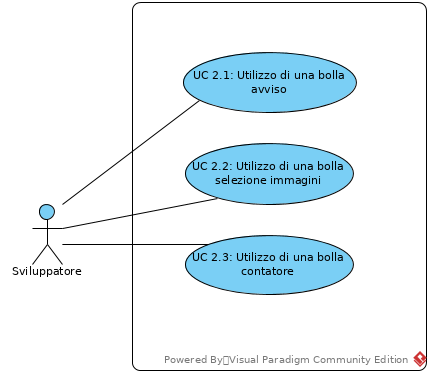
\includegraphics[scale=0.60]{Usecases/img/UC2.png}
	\caption{Caso d'uso UC 2: Modifica del comportamento di una bolla predefinita.}
\end{figure}

\FloatBarrier
\begin{itemize}
\item \textbf{Attori:} Sviluppatore.
\item \textbf{Descrizione:} Lo sviluppatore vuole creare una nuova bolla, modificandone o estendendone una già esistente. In particolare vuole:
	\begin{itemize}
	\item{Aggiungere dei metodi a una bolla.}
	\item{Aggiungere campi dati a una bolla.}
	\item{Sovrascrivere/ridefinire un metodo di una bolla.}
	\end{itemize}
\item \textbf{Precondizione:} Lo sviluppatore vuole creare una nuova bolla, modificandone o estendendone una già esistente. 
\item \textbf{Postcondizione:} Lo sviluppatore ha creato una nuova bolla ed è stata inserita nella libreria di \progetto.
\item \textbf{Scenario principale:}
	\begin{itemize}
	\item{Aggiunta di un metodo ad una bolla (UC 2.1).} 
	\item{Aggiunta di un campo dati ad una bolla (UC 2.2).}
	\item{Sovrascrittura/ridefinizione di un metodo di una bolla (UC 2.3).}
	\end{itemize}
\end{itemize}